%-------------------------
% Resume in Latex
% Author : Zakaria TOZY
%------------------------

\documentclass[11pt,a4paper]{article}

\usepackage{latexsym}
\usepackage[empty]{fullpage}
\usepackage{titlesec}
\usepackage{marvosym}
\usepackage[usenames,dvipsnames]{color}
\usepackage{verbatim}
\usepackage{enumitem}
\usepackage[hidelinks]{hyperref}
\usepackage{fancyhdr}
\usepackage[english,french]{babel}
\usepackage{tabularx}
\usepackage[utf8]{inputenc}
\usepackage[left=0.5in, right=0.5in, top=0in, bottom=0.5in]{geometry}
\usepackage{exscale}  % Pour la commande \HUGE

\usepackage{fontawesome}
\usepackage[scale=0.90,lf]{FiraMono}

\definecolor{light-grey}{gray}{0.83}
\definecolor{dark-grey}{gray}{0.3}
\definecolor{text-grey}{gray}{.08}

\DeclareRobustCommand{\ebseries}{\fontseries{eb}\selectfont}
\DeclareTextFontCommand{\texteb}{\ebseries}

\usepackage{contour}
\usepackage[normalem]{ulem}
\renewcommand{\ULdepth}{1.8pt}
\contourlength{0.8pt}
\newcommand{\myuline}[1]{%
  \uline{\phantom{#1}}%
  \llap{\contour{white}{#1}}%
}

\usepackage{tgheros}
\renewcommand*\familydefault{\sfdefault} 
\usepackage[T1]{fontenc}

\usepackage{graphicx}

\pagestyle{fancy}
\fancyhf{} 
\fancyfoot{}
\renewcommand{\headrulewidth}{0pt}
\renewcommand{\footrulewidth}{0pt}

\urlstyle{same}

\raggedbottom
\raggedright
\setlength{\tabcolsep}{0in}

\titleformat{\section}{
    \bfseries \vspace{-4pt} \raggedright \normalsize
}{}{0em}{}[\color{light-grey} {\titlerule[1pt]} \vspace{-2pt}]

\newcommand{\resumeItem}[1]{
  \item\footnotesize{
    {#1 \vspace{-1pt}}
  }
}

\newcommand{\resumeSubheading}[4]{
  \vspace{2pt}\item
    \begin{tabular*}{\textwidth}[t]{l@{\extracolsep{\fill}}r}
      {\footnotesize\textbf{#1}} & {\footnotesize#2} \\
      {\footnotesize\textit{#3}} & {\footnotesize\textit{#4}} \\
    \end{tabular*}\vspace{2pt}
}

\newcommand{\resumeProjectHeading}[2]{
  \item
  {\footnotesize\textbf{#1}} \hfill {\footnotesize\textit{#2}}
}

\newcommand{\resumeSubItem}[1]{\resumeItem{#1}\vspace{-4pt}}

\renewcommand\labelitemii{$\vcenter{\hbox{\tiny$\bullet$}}$}

\newcommand{\resumeSubHeadingListStart}{\begin{itemize}[leftmargin=0in, label={}]}
\newcommand{\resumeSubHeadingListEnd}{\end{itemize}}
\newcommand{\resumeItemListStart}{\begin{itemize}[label={\textbullet}]}
\newcommand{\resumeItemListEnd}{\end{itemize}\vspace{0pt}}

\color{text-grey}

\begin{document}

\begin{flushleft}
  \begin{minipage}[c]{0.2\textwidth}
    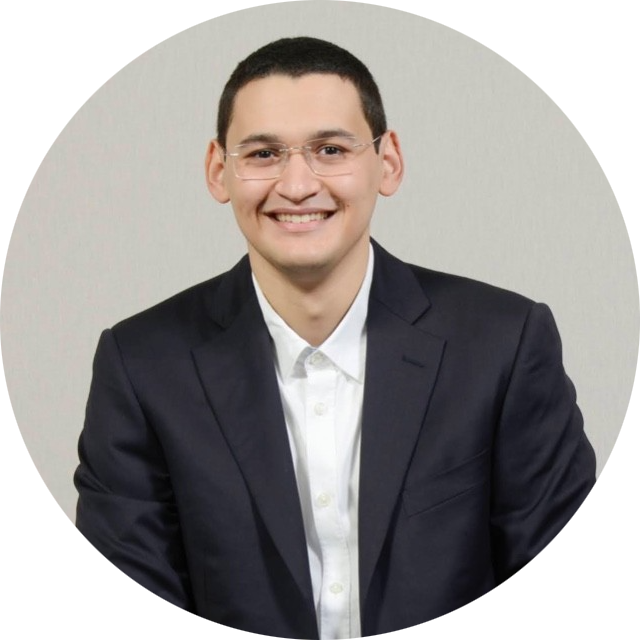
\includegraphics[width=3cm]{images/profilpicture.png}
  \end{minipage}%
  \begin{minipage}[c]{0.8\textwidth}
    {\Huge \textbf{Zakaria TOZY}} \\[2pt]
    {\Large \textbf{Data Engineer | Software Engineer }}
  \end{minipage}
\end{flushleft}

\vspace{-8pt}

\begin{center}
    \small \faPhone\ \texttt{0617407077} \hspace{1pt} $|$
    \hspace{1pt} \faEnvelope\ \texttt{zakaria.tozy@icloud.com} \hspace{1pt} $|$
    \hspace{1pt} \faLinkedin\ \texttt{zakaria-tozy} \hspace{1pt} $|$
    \hspace{1pt} \faMapMarker\ \texttt{Paris} \hspace{1pt} $|$
    \hspace{1pt} \faGithub\ \texttt{zack242} \\ \vspace{0pt}
\end{center}

\begin{itemize}[leftmargin=0in, label={}]
\footnotesize{\item{
Ingénieur diplômé d'un double cursus en systèmes d'information et data science, passionné par la data, l'intelligence artificielle et les technologies innovantes. Enrichi d'une expérience significative en tant que Data Engineer et Data Analyst chez AXA IM, je suis à la recherche d'un CDI pour valoriser et approfondir mes compétences techniques.
}}
\end{itemize}

\section{COMPETENCES}
\begin{itemize}[leftmargin=0in, label={}]
\footnotesize{\item{
{\footnotesize\textbf{Programmation}:} {\footnotesize Python, SQL, Java, JavaScript} \\
\vspace{3pt}
{\footnotesize\textbf{Machine Learning}:} {\footnotesize Scikit-Learn, Pandas, Numpy, NLP, LLM} \\
\vspace{3pt}
{\footnotesize\textbf{Devops}:} {\footnotesize Docker, CI/CD, Git} \\
\vspace{3pt}
{\footnotesize\textbf{Soft Skills}:} {\footnotesize Autonome, Rigoureux, Fort esprit d'analyse} \\
\vspace{3pt}
{\footnotesize\textbf{Langues}:} {\footnotesize Français (Bilingue), Arabe (Bilingue), Anglais (Professionnel - TOEIC 875)} \\
\vspace{3pt}
{\footnotesize\textbf{Data \& Cloud Engineering}:} {\footnotesize PySpark, Databricks, Snowflake, Azure, GCP, S3, dbt}
}
}
\end{itemize}

\section{FORMATIONS}
\resumeSubHeadingListStart
    \resumeSubheading
      {École Centrale d'Électronique (ECE Paris)}
      {Janvier 2024}
      {Ingénieur en Systèmes d'Information et Big Data Analytics}
      {Top 5\% de la promotion}
      \resumeItemListStart
        \resumeItem{Programmation, Bases de données, Électronique}
      \resumeItemListEnd
    \resumeSubheading
      {Institut Polytechnique de Paris (École Polytechnique)}
      {Janvier 2024}
      {Master 2 en Data Sciences}
      {Mention Très bien}
      \resumeItemListStart
        \resumeItem{Machine Learning, Big Data, Cloud Infrastructure, Deep Learning, NLP}
      \resumeItemListEnd
  \resumeSubHeadingListEnd

\section{EXPERIENCES}
\resumeSubHeadingListStart
    \resumeSubheading
      {Projet Personnel}{Février 2024 -- Juin 2024}
      {Ingénieur Blockchain - Développement d'un sniper bot en Rust}{Paris}
      \resumeItemListStart
        \resumeItem{Monitoring de toutes les pools de liquidité de la blockchain Solana.}
        \resumeItem{Mise en place d'un système pour acheter ces tokens dès leur création en moins de 1 seconde.}
        \resumeItem{Automatisation de la revente des tokens après réalisation d'une plus-value.}
      \resumeItemListEnd
    \resumeSubheading
      {AXA Investment Managers - AXA IM}{Août 2023 -- Janvier 2024}
      {Stage de Fin d'Études - Data Engineer / Data Analyst}{Paris}
      \resumeItemListStart
        \resumeItem{Conception et mise en place de pipelines de données pour l'ingestion et la gestion des données métiers.}
        \resumeItem{Optimisation du modèle de données et migration des pipelines de distribution pour le reporting financier.}
        \resumeItem{Tests de nouveaux clusters Databricks et création d'un PoC pour l'anonymisation des données sensibles.}
        \resumeItem{Création de tableaux de bord et calcul des KPIs pour la vision distribuée (ME, OV, CIS, FX).}
      \resumeItemListEnd
    \resumeSubheading
      {Kalima Blockchain et IoT}{Avril 2022 -- Août 2022}
      {Stage - Software Engineer}{Paris}
      \resumeItemListStart
        \resumeItem{Développement d'un explorateur de blockchain propriétaire Kalima en Java/LevelDB.}
        \resumeItem{Implémentation de nouvelles fonctionnalités d'administration pour la blockchain Kalima en Node.js.}
        \resumeItem{Conception et développement d'un système d'authentification multisignature pour les DApps (Decentralized Applications).}
      \resumeItemListEnd
  \resumeSubHeadingListEnd

\section{PROJETS}
\resumeSubHeadingListStart
    \resumeProjectHeading
      {Pipeline d'Analyse Blockchain} {Septembre 2024}
      \resumeItemListStart
        \resumeItem{Création d'une solution cloud pour l'analyse des transactions Bitcoin}
        \resumeItem{Conception et implémentation d'un pipeline de données moderne (Python, SQL, Airflow, dbt, Snowflake)}
      \resumeItemListEnd
    \resumeProjectHeading
      {Analyse en Temps Réel des Réseaux Sociaux} {Avril 2023}
      \resumeItemListStart
        \resumeItem{Création d'une plateforme d'analyse des tendances et sentiments sur Twitter en temps réel}
        \resumeItem{Développement d'un système de classification par topics avec Kafka}
        \resumeItem{Implémentation d'un algorithme de clustering KNN pour la détection de tendances émergentes}
      \resumeItemListEnd
    \resumeProjectHeading
      {Système Multi-Agents IA} {Novembre 2024}
      \resumeItemListStart
        \resumeItem{Développement d'un système conversationnel innovant basé sur deux agents IA autonomes}
        \resumeItem{Intégration de l'API OpenAI pour la génération de réponses contextuelles et pertinentes}
        \resumeItem{Déploiement sur Twitter permettant aux agents d'interagir avec les utilisateurs en temps réel}
      \resumeItemListEnd
\resumeSubHeadingListEnd


\end{document} 